\chapter{Marco Teórico y Antecedentes}
\label{chap:marco_teorico}

El presente capítulo profundiza en la comprensión del comportamiento sedentario (CS), un fenómeno que incide de manera significativa en la calidad de vida relacionada con la salud (CVRS). Se definen conceptos clave, se analizan sus efectos multifacéticos en la salud y se examinan las herramientas actuales para evaluarlos, incluyendo cuestionarios de autoinforme y tecnologías avanzadas. Además, se aborda la integración de variabilidad de la frecuencia cardiaca (HRV) como biomarcador y el papel de la inteligencia artificial (IA) y la lógica difusa (FL) en el análisis de datos biomédicos.

% ============================================================================
\section{Marco Teórico}
\label{sec:marco_teorico}
% ============================================================================

\subsection{Definición de Sedentarismo}
\label{subsec:definicion_sedentarismo}

El sedentarismo se refiere a un estilo de vida donde prevalece uno o varios CS que se prolongan de forma regular, y que requieren de poca o ninguna Actividad Física (AF) \citep{Tremblay2010Physiological}. Además, el concepto de Sedentarismo no excluye la práctica del Ejercicio Físico (EF), de forma que una persona puede ser considerada Sedentaria aun si llegara a practicar EF, pero sin llegar a cumplir las recomendaciones de la Organización Mundial de la Salud (OMS), siendo que se dedica mucho tiempo invertido en conductas sedentarias y prevalece una estimación de gasto calórico total diario muy bajo.

\subsection{Definición del Comportamiento Sedentario}
\label{subsec:definicion_cs}

El CS se refiere a cualquier comportamiento realizado por el individuo en posición acostado, reclinado, sentado o de pie, mientras se está despierto, sin ambulación en dependencia de un bajo gasto energético \citep{Tremblay2017Terminology}. Como ejemplo, mientras se está sentado, reclinado o acostado, cuando se hace uso de dispositivos electrónicos, mientras se lee, o se está escribiendo, también cuando se va sentado en el autobús, automóvil o tren. De pie en una fila, de pie en la iglesia, de pie para una conversación de pasillo, y al usar un escritorio de pie, se consideran comportamientos sedentarios o estáticos. Por tanto, el CS se refiere a las actividades que no aumentan el gasto de energía sustancialmente por encima del nivel de reposo, con un gasto energético inferior a 1,5 Unidades Metabólicas Equivalentes (MET) \citep{Pate2008Terminology,Alvarez2020Sedentarismo}.

Es importante mencionar que esta definición no es la única, el CS se puede categorizar de varias maneras, según la duración, intensidad, frecuencia y cantidad total de AF \citep{Tremblay2017Terminology}.

\subsection{Diferencia entre Comportamiento Sedentario e Inactividad Física}
\label{subsec:diferencia_cs_inactividad}

Es importante mencionar que el CS puede tener un impacto negativo en la salud, incluso en personas que cumplen con las recomendaciones de AF propuestas por la OMS. En otras palabras, paradójicamente, en la actualidad es posible cumplir con las recomendaciones de AF mediante EF y también presentar tiempos sedantes superiores a 8 horas por día, es decir, ser ``físicamente activo pero sedentario'' \citep{ReyesMolina2023Sedentarismo}.

En la actualidad, se emplea el término sedentario o con alto CS para referirse a individuos que prolongan actividades con bajo gasto energético \citep{Tremblay2017Terminology}. Además, para referirse a personas sedentarias, se suele utilizar el término de persona con inactividad física o que es inactiva físicamente, cuando un individuo con un nivel de AF es insuficiente para cumplir con las recomendaciones actuales de AF propuesta por la OMS.

\subsection{Directrices de la OMS sobre Actividad Física}
\label{subsec:directrices_oms}

Las últimas instrucciones que se enmarcan en las Directrices de AF y Hábitos Sedentarios del año 2020, la OMS ponen énfasis en que ``cada movimiento cuenta'', se menciona que para reducir el CS es importante la promoción de la actividad física incidental ya que puede ayudar a incrementar gradualmente la AF realizada en un día hacia cantidades recomendadas para una salud óptima. No obstante, las recomendaciones de AF son las siguientes.

Para niños y adolescentes se recomienda realizar al menos una media de 60 minutos de AF diaria principalmente aeróbica de intensidad moderada a vigorosa a lo largo de la semana.

Los adultos deben acumular a lo largo de la semana un mínimo de entre 150 y 300 minutos de AF aeróbica de intensidad moderada, o bien un mínimo de entre 75 y 150 minutos de AF aeróbica de intensidad vigorosa, o bien una combinación equivalente de actividades de intensidad moderada y vigorosa, con el fin de obtener beneficios notables para la salud.

Por último, las personas mayores (a partir de 65 años) pueden realizar la AF como actividad recreativa o de ocio (juegos, deportes o ejercicios programados) y en el marco de los desplazamientos (caminar e ir en bicicleta o en algún otro medio rodado), el trabajo o los que haceres domésticos, en el contexto ocupacional, educativo, doméstico y comunitario cotidiano \citep{Bull2020,WHO2020GuidelinesAnnex}.

\subsection{Actividad Física y Ejercicio Físico}
\label{subsec:af_ef}

La AF y el EF, aunque a menudo se usan indistintamente y son términos son ampliamente utilizados para describir el movimiento humano, es relevante destacar que estos no son sinónimos, y sus definiciones difieren.

La AF es cualquier movimiento corporal producido por la contracción del músculo esquelético que aumenta el gasto energético por encima de un nivel basal \citep{Caspersen1985PhysicalActivity}. No obstante, también existen actividades físicas incidentales, como parte de las actividades físicas de la vida diaria que no posee estructura, no requiere compromiso de tiempo, y no tiene propósitos de salud, fines recreativos o del Principio FITT (i.e., Frecuencia, Intensidad, Tiempo, Tipo). Entre ellas, las realizadas en el hogar, trabajo, estudio y tiempo libre; como el uso de escaleras, desplazamientos activos, estar de pie, ir de compras, jardinería o tareas domésticas, AF ocupacional, actividades lúdicas con niños, paseo de mascotas, entre otras \citep{ReyesMolina2023Sedentarismo}.

El ejercicio es una subcategoría de la AF que es ``planificada, estructurada, repetitiva e intencional en el sentido de que el objetivo es mejorar o mantener uno o más componentes de la aptitud física''. El ejercicio y el entrenamiento físico se utilizan con frecuencia de manera indistinta y general, se refieren a la AF realizada con el propósito de mejorar o mantener la condición física, el rendimiento físico o la salud \citep{Caspersen1985PhysicalActivity}.

\subsection{Condición Física Relacionada con la Salud}
\label{subsec:condicion_fisica}

Es necesario diferenciar la condición física que se relaciona con el rendimiento, de la condición física relacionada con la salud. Esta última, está determinada por la resistencia cardiorrespiratoria, la fuerza y resistencia muscular, la flexibilidad y la composición corporal. Mientras que la Condición Física relacionada con el Rendimiento lo está, por los factores relacionados con la salud más la coordinación, potencia, velocidad y equilibrio.

Por tanto, la Condición Física Relacionada con la Salud representa el estado de los sistemas metabólicos y de las variables predictoras para el riesgo de morbilidad y mortalidad, las cuales pueden alterarse de manera favorable al aumentar la AF o el EF regular sin que se produzca un aumento en el Volumen Máximo de Oxigeno ($\mathrm{VO}_{2\text{máx}}$) relacionado con el entrenamiento \citep{Riebe2018ACSM}.

\subsection{Actividad y Capacidad Aeróbica}
\label{subsec:actividad_capacidad_aerobica}

La actividad aeróbica (también llamada resistencia o actividad cardiovascular), ocurre cuando los músculos grandes se mueven de manera rítmica durante un período sostenido. La actividad aeróbica hace que la Frecuencia Cardiaca (FC) aumente y que la respiración se vuelva más dificultosa. La AF aeróbica tiene 3 componentes: intensidad, frecuencia y duración. La intensidad describe el esfuerzo con el que una persona trabaja para realizar la actividad. Las intensidades más estudiadas son moderadas (equivalentes en esfuerzo a caminar a paso ligero) y vigorosas (equivalentes en esfuerzo a correr o trotar). La frecuencia describe la frecuencia con la que una persona realiza actividad aeróbica. La duración describe cuánto tiempo una persona realiza una actividad \citep{Piercy2018Guidelines}.

La capacidad aeróbica es una de las características más relacionada con la salud, debido a que representa una de las cualidades más importantes de la condición física. La ejecución de la actividad aeróbica requiere principalmente del estado funcional de los sistemas respiratorio, locomotor y cardiovascular \citep{Riebe2018ACSM}. La capacidad aeróbica o funcional, constituye una medida directa del grado general de salud ya que refleja la capacidad de funcionamiento del sistema cardiorrespiratorio, metabólico y respiratorio \citep{Gonzalez2018CapacidadAerobica,Riebe2018ACSM}.

\subsection{Frecuencia Cardiaca}
\label{subsec:frecuencia_cardiaca}

El control de la FC es el método más popular y sencillo de controlar la intensidad de la AF. Para ello se valora la FC de reposo y la Frecuencia Cardiaca Máxima ($\text{FC}_{\text{máx}}$) definida como el número máximo de latidos que puede realizar el corazón durante un minuto. Su utilidad se debe a la correlación relativamente lineal existente entre la FC y la intensidad del esfuerzo, valorada mediante el consumo de oxígeno expresado como $\mathrm{VO}_{2\text{máx}}$ o también con los METs \citep{Abellan2014Prescripcion}.

En seguida, se muestran varias fórmulas de estimación, algunas son menos conocidas, pero todas están avaladas por estudios científicos que demuestra su validez, reproducibilidad y confiabilidad.

\subsubsection{Fórmula de Fox \& Haskell}
\label{subsubsec:formula_fox_haskell}

Propuesta por la ACSM's expone la estimación de la $\text{FC}_{\text{máx}}$ de la siguiente manera \citep{Fox1968HeartRate}:

\begin{equation}
\text{FC}_{\text{máx}} \text{ (estimada)} = 220 - \text{edad (en años)}
\label{eq:fox_haskell}
\end{equation}

\subsubsection{Fórmula de Tanaka}
\label{subsubsec:formula_tanaka}

Recomendada para el trabajo de personas mayores \citep{Tanaka2001AgePredicted}, ya que sus autores consideran que la fórmula de la ACSM's $\text{FC}_{\text{máx}}$ infravalora las pulsaciones reales en estas edades la fórmula es la siguiente:

\begin{equation}
\text{FC}_{\text{máx}} \text{ (estimada)} = 208 - (0.7 \times \text{edad})
\label{eq:tanaka}
\end{equation}

\subsubsection{Fórmula de Karvonen}
\label{subsubsec:formula_karvonen}

Desarrollada por el fisiólogo finlandés Martti Karvonen en 1957, es una herramienta sencilla y ampliamente utilizada para estimar la intensidad de trabajo aeróbico durante el ejercicio. Esta fórmula se basa en la Frecuencia Cardíaca en Reposo ($\text{FC}_{\text{r}}$) medida en posición de bipedestación y la $\text{FC}_{\text{máx}}$ de un individuo para determinar la que zona de intensidad según la FC objetivo para la AF \citep{Abellan2014Prescripcion}.

La fórmula de Karvonen se utiliza para establecer diferentes zonas de intensidad de entrenamiento:

\begin{itemize}
    \item Zona de baja intensidad (40--60\%)
    \item Zona de intensidad moderada (60--70\%)
    \item Zona de alta intensidad (70--80\%)
    \item Zona de intensidad máxima ($>$80\%)
\end{itemize}

\begin{equation}
\text{FC}_{\text{obj}} = \text{FC}_{\text{r}} + (\text{FC}_{\text{máx}} - \text{FC}_{\text{r}}) \times \text{Int.}
\label{eq:karvonen}
\end{equation}

\subsection{Variabilidad de la Frecuencia Cardiaca (HRV)}
\label{subsec:hrv}

La variabilidad de la frecuencia cardíaca (HRV) representa las fluctuaciones en el tiempo entre latidos consecutivos del corazón \citep{TaskForce1996HeartRate,Quigley2024HeartRate}. Estas variaciones son controladas por el sistema nervioso autónomo, lo que convierte a la HRV en un biomarcador no invasivo y continuo del estado autonómico del individuo \citep{Tefera2024HeartRate,Trimmel2015ApplicationWearable}. Una HRV alta generalmente se asocia con un buen estado de salud y una mayor capacidad de adaptación fisiológica, mientras que una HRV baja puede indicar estrés, fatiga o condiciones de salud subyacentes. El parámetro HRV-SDNN (desviación estándar de los intervalos NN) es una métrica común para cuantificar la HRV \citep{Damoun2024HeartRate,Laborde2017HeartRate}, proporcionando información valiosa sobre el equilibrio entre los sistemas simpático y parasimpático. La integración de la HRV permite un monitoreo más dinámico y sensible de la respuesta fisiológica a la actividad física y el sedentarismo, ofreciendo una visión más completa del bienestar general \citep{Bonneval2025PhysicalActivity,Fuller2021ReliabilityHRV,Szulc2023HeartRate,AppleWatchHRV2024}.

\subsection{MET (Equivalente Metabólico)}
\label{subsec:met}

Un MET es la cantidad de oxígeno necesaria para el mantenimiento durante 1 minuto de las funciones metabólicas del organismo con el individuo en reposo y sentado, equivalente a 3,5 ml$\times$kg$\times$min. Además, el MET se utiliza para proporcionar la relación entre la tasa de energía gastada durante una actividad y la tasa de energía gastada en reposo. Los MET son una forma útil, conveniente y estandarizada de describir la intensidad absoluta de las actividades físicas \citep{Riebe2018ACSM}.

La prescripción basada en el coste energético de la actividad mediante MET, es la aplicación más lógica para sujetos aparentemente sanos y aquellos con valores altos de $\mathrm{VO}_{2\text{máx}}$, pero resulta menos aplicable en personas con ENT o en individuos con baja capacidad funcional \citep{Abellan2014Prescripcion}.

La variable $\mathrm{VO}_{2\text{máx}}$ es el producto del gasto cardíaco o débito cardíaco máximo (D $\cdot$ lt sangre $\cdot$ mín.$^{-1}$) y la diferencia arteriovenosa de oxígeno (mlO$_2$ $\cdot$ lt sangre $^{-1}$), se expresa típicamente en términos relativos (ml $\cdot$ kg $^{-1}$ $\cdot$ min $^{-1}$) en lugar de absolutos (ml $\cdot$ min $^{-1}$), lo que permite comparaciones significativas entre individuos con diferente peso corporal. La variación significativa en $\mathrm{VO}_{2\text{máx}}$ entre poblaciones y niveles de condición física se debe principalmente a diferencias en gasto cardiaco máximo (D) por lo tanto, el $\mathrm{VO}_{2\text{máx}}$ está estrechamente relacionado con la capacidad funcional del corazón.

\subsection{Dispositivos y Tecnologías Electrónicas Portátiles}
\label{subsec:dispositivos_wearables}

Actualmente se habla de que vivimos una ``cuarta revolución industrial'' o una ``cuarta revolución tecnológica'' la cual precede a la era de la microelectrónica, las tecnologías de la información, tecnologías de las comunicaciones y por supuesto a la World Wide Web (internet). Lo que ha derivado en grandes innovaciones surgidas, que van desde la digitalización, el manejo de grandes volúmenes de información (Big data), la IA, la robótica, las neurociencias y la biotecnología, entre otras \citep{Martinez2020Tecnologias}.

La Comisión Electrotécnica Internacional (IEC) es una organización líder en el desarrollo de normas internacionales para la electro-tecnología. Sus normas son utilizadas por millones de personas en todo el mundo para garantizar la seguridad, la eficiencia y la interoperabilidad de los productos eléctricos, electrónicos y relacionados.

De acuerdo con la IEC, para el uso de la palabra ``Wearables'' del inglés que se utiliza comúnmente para referirse a los ``dispositivos y tecnologías electrónicas portátiles'' se refiere a un amplio rango de dispositivos electrónicos que se pueden llevar puestos o integrados en la ropa u otros objetos.

La IEC define el alcance del Comité Técnico 124 (TC 124) como la ``estandarización en el campo de los dispositivos y tecnologías electrónicas portátiles'' e incluye; Materiales y dispositivos adheribles: Estos son dispositivos electrónicos delgados y flexibles que se pueden adherir a la piel u otras superficies. Materiales y dispositivos implantables, se trata de dispositivos electrónicos que se colocan quirúrgicamente debajo de la piel o dentro del cuerpo. Materiales y dispositivos ingeribles, son dispositivos electrónicos que se pueden tragar y viajar a través del sistema digestivo para realizar mediciones o administrar medicamentos. Materiales y dispositivos textiles electrónicos, se trata de textiles que incorporan componentes electrónicos, lo que les otorga nuevas funcionalidades \citep{IEC2019Wearables}.

\subsection{Sensores integrados en dispositivos portátiles}
\label{subsec:sensores}

\subsubsection{Acelerómetro}
\label{subsubsec:acelerometro}

Un acelerómetro es un sensor de chip que está formado por un elemento capacitivo microelectromecánico, y piezoeléctrico que detecta el cambio en la aceleración de una pequeña masa en el sensor, como el que se muestra en la \Cref{fig:acelerometro_mma7361}, el cual es un dispositivo que mide la fuerza estática que incluye la gravedad, y la fuerza dinámica que puede incluir vibraciones y movimiento. La forma en que mide es en metros por segundo al cuadrado (m/s²) o por la fuerza G (g) que mide la aceleración de la gravedad.

\begin{figure}[htbp]
    \centering
    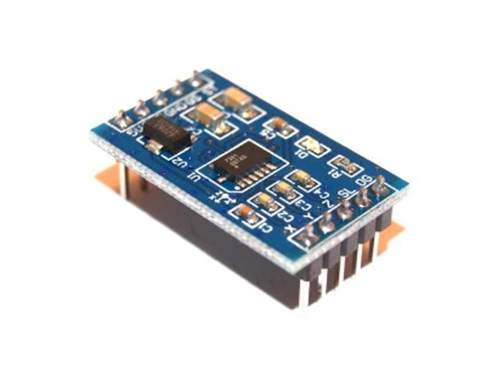
\includegraphics[width=0.5\textwidth]{figuras/acelerometro_modelo_MMA7361.png}
    \caption{Módulo de sensor tipo acelerómetro modelo MMA7361}
    \label{fig:acelerometro_mma7361}
\end{figure}

\subsubsection{Fotopletismografía}
\label{subsubsec:fotopletismografia}

La Fotopletismografía (PPG) es una técnica ampliamente usada para medir la (FC) y la saturación de oxígeno en sangre (SpO$_2$) de manera no invasiva. Como ejemplo en la \Cref{fig:ppg_adpd1081} se muestra el sensor óptico PPG modelo ADPD1081 que está basado en un sistema optoelectrónico formado por un diodo emisor de luz LED y un elemento fototransistor que funciona como receptor y que en conjunto se encargan de iluminar la piel, y detectar las variaciones lumínicas que se producen debido a los efectos de reflexión y absorción de la luz por la sangre en los vasos sanguíneos \citep{Torres2023Fotopletismografia}.

\begin{figure}[htbp]
    \centering
    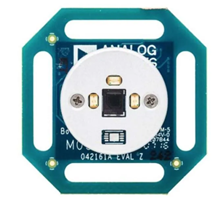
\includegraphics[width=0.5\textwidth]{figuras/PPG_modelo_ADPD1081.png}
    \caption{Sensor óptico PPG modelo ADPD1081}
    \label{fig:ppg_adpd1081}
\end{figure}

La FC y el $\mathrm{VO}_{2\text{máx}}$ tienden a estar linealmente relacionados en una gran parte del rango de trabajo aeróbico. Cuando se conoce esta relación, la FC del ejercicio puede ser utilizada para estimar el $\mathrm{VO}_{2\text{máx}}$, y luego calcular el gasto de energía durante las actividades de la vida diaria. \citet{Rodriguez2021MonitoresFitness} mencionan que las ventajas que presenta este método son: información acerca de la intensidad duración y frecuencia, por lo cual es adecuado para la mayoría de las personas, relativamente económico y permite un análisis fácil y rápido de los datos.

\subsection{Inteligencia Artificial para el Reconocimiento del Comportamiento Sedentario}
\label{subsec:ia_reconocimiento_cs}

En el contexto de las ciencias de la computación, la IA se refiere a una disciplina y un conjunto de capacidades cognoscitivas e intelectuales expresadas por sistemas informáticos o combinaciones de algoritmos cuyo propósito es la creación de máquinas que imiten la inteligencia humana para realizar tareas, y que pueden mejorar conforme recopilen información. Sin embargo, durante la última década, la investigación de la IA en el ámbito de la salud y la medicina ha comenzado a mostrar resultados prometedores y aplicaciones prácticas, como la detección totalmente automática de nuevos biomarcadores para el diagnóstico clínico \citep{Farrahi2024ArtificialIntelligence}. La IA ha sido reconocida como una fuerza productiva y disruptiva en la atención médica llegando a considerarla como una herramienta innovadora con el potencial de impactar en las prácticas clínica \citep{Santos2021ArtificialIntelligence,SyedAbdul2020ArtificialIntelligence}.

La tecnología portátil y los sensores están emergiendo como herramientas prometedoras para el monitoreo continuo y en tiempo real de la salud. Desde relojes inteligentes hasta rastreadores de AF y ropa conectada a Internet, los dispositivos portátiles equipados con sensores permiten a los usuarios medir y analizar datos relacionados con su estado fisiológico, actividades y bienestar general. Los rastreadores de AF contienen acelerómetros y monitores ópticos de fotopletismografía ya son ampliamente utilizados por los consumidores para contar pasos y controlar la frecuencia cardíaca durante el ejercicio, estos sensores portátiles son de grado clínico para medir con precisión los signos vitales. Por ejemplo, la Presión Arterial (PA), la Frecuencia Respiratoria (FR), (SpO$_2$), la temperatura de la piel, y más. La integración inalámbrica y los algoritmos de IA permiten que los dispositivos portátiles realicen un seguimiento de los indicadores de salud las 24 horas del día, los 7 días de la semana y proporcionen comentarios a los usuarios \citep{Khan2024ArtificialIntelligence}.

\subsection{Teoría de lógica difusa para el análisis de datos biométricos}
\label{subsec:teoria_logica_difusa}

La teoría de FL, desarrollada inicialmente por Lotfi Zadeh en 1965, se basa en la idea de que la verdad no siempre es una cuestión de blanco o negro, sino que puede estar en un espectro de grises. A diferencia de la lógica clásica, que trabaja con valores binarios (0 o 1), la FL permite valores intermedios, lo que la hace especialmente útil para manejar información imprecisa, vaga o incierta. Se ha demostrado que los sistemas difusos son aproximadores universales, esto se debe al isomorfismo entre dos álgebras; Un álgebra abstracta (que trata con grupos, campos y anillos) y un álgebra lineal (que maneja espacios vectoriales, vectores de estado y matrices de transición). Este isomorfismo refleja la estructura de un sistema difuso, que comprende una implicación entre acciones y conclusiones (antecedentes y consecuentes). Así como una función algebraica mapea una variable de entrada a una variable de salida, un sistema difuso mapea un grupo de entrada a un grupo de salida, que pueden ser proposiciones lingüísticas u otras formas de información difusa \citep{Ross2010FuzzyLogic}.

La base sobre la cual se asienta la teoría de sistemas difusos es un teorema fundamental del análisis real en álgebra conocido como el teorema de Stone-Weierstrass, desarrollado inicialmente por Weierstrass en 1885 y simplificado por Stone en 1937. Este teorema establece que cualquier función continúa definida en un intervalo cerrado puede ser aproximada tan cerca como se desee por una función polinómica \citep{Ross2010FuzzyLogic,Gupta2011FuzzyLogic}. Los sistemas difusos, aprovechando este principio, tienen la capacidad de aproximar comportamientos de sistemas donde las funciones analíticas o las relaciones numéricas no existen.

Los sistemas difusos son particularmente útiles en dos contextos generales: Primero en situaciones que involucran sistemas altamente complejos cuyos comportamientos no se entienden completamente. Segundo en situaciones donde una solución aproximada pero rápida es suficiente. Estos sistemas tienen un alto potencial para comprender sistemas complejos, tales como sistemas biológicos o médicos, donde la relación entre causas y efectos no se entienden completamente, pero pueden observarse \citep{Kaur2022FuzzyLogic}.

\subsection{Síntesis del Marco Conceptual}
\label{subsec:sintesis_marco_conceptual}

El marco teórico presentado establece la base conceptual para comprender la compleja interacción entre el comportamiento sedentario, la actividad física y la calidad de vida relacionada con la salud. La revisión de las definiciones, las directrices de la OMS y las tecnologías de monitoreo resalta la necesidad de enfoques innovadores. Las bases conceptuales para un modelo híbrido que integra mediciones objetivas de comportamiento sedentario, biomarcadores autonómicos continuos y herramientas de inteligencia artificial. La integración de la variabilidad de la frecuencia cardíaca y la aplicación de la lógica difusa emergen como elementos clave para el desarrollo de un modelo más preciso y adaptable, capaz de capturar la dinámica de estas interacciones en contextos de vida real.

% ============================================================================
\section{Antecedentes}
\label{sec:antecedentes}
% ============================================================================

En esta sección de antecedentes se enmarca la problemática actual que representa el comportamiento sedentario, y las principales motivaciones para realizar esta investigación. Se presentan los elementos básicos que permiten estudiar los patrones de CS y la percepción de la CVRS. Asimismo, se aborda la implementación IA al análisis de datos obtenidos de sensores biométricos en monitores de AF, portables de consumo público.

\subsection{Impacto del Comportamiento Sedentario}
\label{subsec:impacto_cs}

El CS es un factor de riesgo importante para una serie de Enfermedades No Transmisibles (ENT), incluyendo obesidad, enfermedades del corazón, diabetes tipo 2, accidentes cerebrovasculares, algunos tipos de cáncer, depresión y falta de sueño. Actualmente, el CS se contempla como parte de una Sindemia Global, lo que lo vuelve difícil de comprender. Existe un nexo entre los Riesgos Dietéticos, el alto Índice de Masa Corporal (IMC), y los Ambientes Obeso-Génicos con el estudio del CS, ya que estos factores combinados aumentan el riesgo de padecer ENT y están directamente relacionados con la Salud, Bienestar y CV de los individuos \citep{Swinburn2019Syndemic}.

La investigación realizada de \citet{Murray2020GlobalBurden}, concluyó que ningún estado perteneciente a la OMS ha tenido una disminución significativa en la proporción de la población con IMC alto, entre 1990 y 2019 o en la última década. Dada la creciente prevalencia del CS en la sociedad moderna y su impacto adverso en la salud, la OMS desde el 2004 en la Asamblea Mundial de la salud emitió la ``Estrategia Mundial de la OMS sobre Dieta, AF y Salud (DPAS por sus siglas en inglés)'', en donde se definía un plan de acción para implementar directrices sobre AF para la salud \citep{Meusel2006StrategiaGlobal}.

A pesar del lanzamiento de la DPAS, ningún país ha revertido significativamente la tendencia al aumento de las tasas de obesidad o diabetes, \citet{Guthold2020GlobalTrends} mencionan que la mayoría de los niños y adolescentes, no cumplen con los requerimientos mínimos de AF y que el CS en menores aumentó significativamente del 2001 al 2016. En los hallazgos de la OMS a través de la Encuesta sobre la capacidad de los países para afrontar las enfermedades no transmisibles (2021), se menciona que casi un tercio de los adultos tampoco alcanzan los niveles recomendados de AF. En México el CS en adultos es mayor llegando al 40\% según la Encuesta Nacional de Salud y Nutrición 2022 \citep{Campos2023ENSANUT}. Asimismo, se estima que, en 2019, las ENT provocaron cinco millones de muertes a nivel global y en la Región de las Américas, las ENT representan casi cuatro de cada cinco muertes anuales \citep{StrategicPlanPAHO2020}. Además, en 2022, aproximadamente 2500 millones de adultos de 18 o más años tenían sobrepeso, igualmente 390 millones de menores padecían de sobrepeso \citep{WHO2022AsambleaMundial}.

Como resultado, muchos países de ingresos bajos y medianos se enfrentan ahora a una carga cada vez mayor de riesgos modernos para la salud a medida que aumenta la esperanza de vida y las principales causas de muerte y discapacidad se desplazan hacia las ENT. Los costos actuales del CS se estiman en alrededor en más de \$300 000 millones de dólares al año a nivel mundial, esto debido a los costos directos de la atención médica y la pérdida de productividad económica \citep{Okunogbe2021EconomicImpact}. Siendo la responsabilidad por la exposición a conductas sedentarias no solo de los individuos, sino también de los gobiernos y los ministerios de salud. Por tanto, la prevención y tratamiento se debe extender a toda la población no solo a los grupos que están clínicamente en alto riesgo de padecer una ENT \citep{WHO2009GlobalRisks}.

La consecución a esta problemática consiste en alcanzar la meta 3.4 de los ODS, que es reducir en un tercio la mortalidad prematura por ENT para 2030. Por consiguiente, se propone el plan de aceleración que se ha desarrollado en consonancia con las recomendaciones dirigidas a fortalecer y vigilar la reducción del CS, y su plazo coincide con la hoja de ruta 2023--2030 relativa a la ejecución del plan de acción mundial para la prevención y el control de las ENT 2013--2030. Aunado a esto en el ``Informe sobre la situación mundial de la AF'' mencionan que en la aplicación del el ``Plan de acción mundial sobre AF 2018--2030 (GAPPA por sus siglas en inglés)'' \citep{WHO2022InformeActividad} la implementación ha sido lenta y desigual. Además, se ofrece una primera visión del impacto de la COVID-19, poniendo de manifiesto la importancia de la AF regular para la salud mental y física.

Recalcando que mientras el mundo sigue respondiendo a la pandemia de COVID-19 y recuperándose de ella, es necesario implementar medidas encaminadas a prevenir conductas sedentarias, que se detallan en las siguientes secciones.

\subsection{Instrumentos de evaluación del Comportamiento Sedentario}
\label{subsec:instrumentos_evaluacion}

Con relación a los sistemas de vigilancia y los instrumentos de evaluación es importante mencionar que hasta hace poco los principales métodos para medir la AF y los comportamientos sedentarios era a través de la auto notificación utilizando materiales de evaluación como el Cuestionario Mundial sobre AF (Global Physical Activity Questionnaire, GPAQ), la Encuesta Mundial de Salud a Escolares (Global Student Health Survey, GSHS) y el cuestionario Health Behaviour in School-aged Children (HBSC) \citep{CDC_GSHS,GPAQ2012AnalysisGuide}. Estos métodos tienen ventajas ampliamente demostradas. Sin embargo, el informe sobre la situación mundial de la AF del 2022 también reconoce una importante laguna en el seguimiento del GAPPA. Entre ellas destaca la ausencia de vigilancia de la AF entre las personas con discapacidad, así como entre los niños menores de nueve años \citep{WHO2022InformeActividad}.

Para poner en contexto en México Ensanut 2022, que es una encuesta probabilística con diseño de muestra polietápico y estratificado, con representatividad nacional y de ocho regiones en México. Para evaluar los niveles de AF en niños de 10--14 años, se utilizó la pregunta ``En los últimos 7 días, ¿Cuántos días estuviste activo durante al menos 60 minutos al día?'' del cuestionario (HBSC). Y aunque este instrumento de evaluación es ampliamente utilizado en México y en el mundo, posee limitaciones como la tendencia al sesgo de notificación (reportar de manera inexacta o incompleta la información) y el error de medición (utilizar instrumentos no adecuados o realizar mal las mediciones) \citep{Romero2022ENSANUT}.

Dado el reconocimiento de estas deficiencias en los sistemas de vigilancia, se propone por parte de la OMS el análisis de las potenciales ventajas que se tienen de recopilar datos de dispositivos portátiles y móviles. Para apoyar en el seguimiento de la AF buscando datos coherentes y congruentes que garanticen la armonía de los datos en su uso y eficiencia. Tomando en cuenta eso, menciona que se necesita un consenso mundial sobre las herramientas técnicas, los protocolos y los obstáculos financieros, para su uso en los sistemas de seguimiento nacionales y mundiales.

\subsection{Cómo afecta el CS en la CVRS}
\label{subsec:cs_afecta_cvrs}

Fomentar estilos de vida activos y saludables permite a la población, una mejor percepción de CVRS, de acuerdo con la investigación realizada por Chaves y cols., la capacidad aeróbica y la CVRS son condiciones que están asociadas a un declive que progresa con la edad y a estilos de vida sedentarios, en su investigación determinaron que la capacidad aeróbica tiende a disminuir a un ritmo entre 5 a 15\% por década, luego que un individuo pasa de los 30 años de edad en personas sedentarias, en contraparte, las personas físicamente activas pueden retener una reserva suficiente de aptitud aeróbica, para mantener la capacidad funcional durante su edad adulta \citep{Chaves2017CapacidadAerobica}.

\subsection{Uso de sensores para el análisis del Comportamiento Sedentario}
\label{subsec:uso_sensores_analisis_cs}

Los monitores de AF más recientes, implementan el uso de sensores, los cuales son un dispositivo de entrada que mide una magnitud o un parámetro físico para proveer una salida que pueda ser manipulada por un sistema \citep{Alvarez2020Sedentarismo}. Los sensores se clasifican de diversas maneras, pero las más comunes son por tipo de variable a medir o por el principio de transducción. Estos son componentes capaces de obtener, medidas fisiológicas, posición, orientación, velocidad etc. de cualquier dispositivo donde sea utilizado.

\subsubsection{Acelerómetros}
\label{subsubsec:acelerometros_analisis}

Dada la creciente preocupación por la salud y el comportamiento sedentario, se han hecho esfuerzos por medir de forma cuantitativa, las predicciones de gasto energético expresado en MET. Intentando categorizar la intensidad de la AF mediante el uso de acelerómetros. En un estudio realizado por \citet{Rothney2008ValidityAccelerometers} se buscó evaluar la exactitud de tres tipos de acelerómetros, ActiGraph, Actical y RT3, donde se implementó un método, que contemplo el uso de una cámara de calorimetría indirecta para validar su precisión. Llegando a la conclusión de que los monitores portátiles basados en acelerometría son un medio factible y objetivo para detectar patrones de comportamiento sedentario.

Sin embargo, los autores reconocen que hay algunas limitaciones en el estudio, como la dificultad para distinguir entre diferentes niveles de actividad. Los acelerómetros pueden tener dificultades para diferenciar entre comportamientos sedentarios muy baja intensidad, como estar sentado sin movimiento, y otros niveles de AF ligera. Esto puede llevar a cierta imprecisión en la clasificación de los periodos de actividad sedentaria.

De la misma forma la sensibilidad a la posición del dispositivo, la colocación del acelerómetro en el cuerpo puede afectar la precisión de las mediciones. Por ejemplo, algunos dispositivos podrían no capturar adecuadamente ciertos movimientos o actividades si no se usan en la posición correcta. Además, las limitaciones en la detección de comportamientos específicos, los acelerómetros pueden tener problemas para detectar ciertos comportamientos sedentarios específicos, como estar de pie sin movimiento o realizar movimientos muy sutiles, sobre todo cuando se utilizan en la muñeca, lo que puede afectar la precisión de las mediciones.

En este contexto, \citet{Henriksen2018UsingSmartphone} indica que la precisión de un dispositivo portátil de seguimiento de AF en comparación con el IPAQ, subestima significativamente la cantidad de AF informada por los participantes. Más sus conclusiones respecto a las limitaciones fueron similares a las del artículo de \citet{Rothney2008ValidityAccelerometers}. Pero igual recomiendan que los médicos y los profesionales de la salud pública sigan utilizando los cuestionarios para medir el CS a la par que los dispositivos portátiles ya que estos pueden ser útiles para algunos propósitos, como monitorear la AF en el día a día.

\subsection{Monitores de Actividad Física Portables de consumo público}
\label{subsec:monitores_af_consumo_publico}

Los dispositivos que se llevan ``puestos'' (wearables) aprovechan los avances en la tecnología para monitorizar los signos vitales y otros parámetros biométricos a través de teléfonos inteligentes o dispositivos que se adosan al cuerpo como un reloj, bandas o ropa. Bhuyan y cols., sugieren que estos dispositivos pueden monitorear e integrar diferentes parámetros importantes para el tratamiento de comorbilidades en pacientes con ENT \citep{Bhuyan2016WearableDevices}. Es así que los esfuerzos de la comunidad de investigación biomédica por la relevancia de los múltiples hallazgos en torno a la medición de la AF, en la actualidad existen cientos de monitores wearables para el consumo público. Los cuales incorporan diferentes sensores, que arrojan múltiples variables fisiológicas, adoptando su uso como una estrategia para promover un estilo de vida activo.

Tal ha sido el impacto de los monitores wearables que las estadísticas proporcionadas en market.us por Scoop en 2023, reportaron que en el mercado mundial de dispositivos de fitness y bienestar digital se generó 19.3 mil millones de dólares en ingresos en 2022. Además, se espera que este mercado crezca a una tasa compuesta anual del 19.1\% entre 2023 y 2030, alcanzando un valor de 182.9 mil millones de dólares. Además, se espera que la penetración de usuarios de estos dispositivos aumente del 9.52\% en 2023 al 10.36\% en 2028 \citep{Tajammul2023WearablesMarket}.

\subsubsection{Validación de los Monitores de Actividad Física Portables}
\label{subsubsec:validacion_monitores_af}

En el artículo de Wright y cols., exploraron el potencial de múltiples dispositivos wearables o monitores de AF portátiles. Estos dispositivos se basan principalmente en sensores de acelerometría para contar pasos y estimar el gasto energético. Si bien se encontró que muchos de estos monitores tienen precisiones similares a los de grado de investigación para contar pasos, existen limitaciones inherentes a la tecnología de acelerometría para estimar con precisión el gasto energético, especialmente en actividades de vida libre que implican movimientos complejos y no cíclicos \citep{Wright2017ValidityWearables}.

Por otro lado, el estudio de Dinesh y cols., se centraron específicamente en validar las estimaciones de gasto energético de los monitores ActiGraph GT1M y GT3X, ampliamente utilizados en investigación. Estos dispositivos también se basan en acelerometría, pero los autores encontraron que el factor determinante en la precisión de las estimaciones era la versión del firmware utilizado, que incluye los algoritmos de procesamiento de la señal de los acelerómetros \citep{Dinesh2014ValidityActiGraph}.

Los hallazgos de ambos estudios se complementan al resaltar las fortalezas y limitaciones de los monitores de AF basados en acelerometría. Los estudios de Wright, Dinesh y cols., demostraron su utilidad para contar pasos, y expusieron las variaciones en las estimaciones de gasto energético dependiendo del firmware y las condiciones en contextos de vida libre \citep{Wright2017ValidityWearables,Dinesh2014ValidityActiGraph}.

Lo que sugiere la necesidad de estandarización y validación constante por parte de los fabricantes. Además, los resultados ponen de manifiesto la necesidad de explorar tecnologías alternativas o complementarias a la acelerometría para superar sus limitaciones en la evaluación del gasto energético en contextos de vida libre \citep{Dinesh2014ValidityActiGraph}. Enfoques prometedores incluyen el uso de sensores de frecuencia cardíaca, temperatura corporal, conductancia eléctrica de la piel, entre otros, en combinación con algoritmos de ML para reconocer patrones de actividad complejos.

Wright, Dinesh y cols., comparten la idea de que los algoritmos utilizados en los monitores de AF de los consumidores para determinar, los pasos dados, la distancia recorrida y el gasto de energía, generalmente no se comparten con los investigadores. Incluso Dinesh y cols., mencionan que los monitores pueden estar utilizando enfoques de reconocimiento de patrones más robustos de lo que se utilizan en su estudio \citep{Wright2017ValidityWearables,Dinesh2014ValidityActiGraph}.

Por su parte Wright y cols., ponen en evidencia que las empresas no solo pueden cambiar sus algoritmos sin previo aviso, sino que es posible que no revelen este hecho después, por lo que es posible que los investigadores ni siquiera sepan sobre esta posible discontinuidad en sus datos a lo largo del tiempo. Además de las actualizaciones de firmware relativamente frecuentes que pueden cambiar los algoritmos, las empresas actualizan continuamente sus dispositivos, lo que hace que los modelos más antiguos queden obsoletos. Dejando a los investigadores en duda de hasta qué punto los estudios previos de validez de un dispositivo se aplicarían a sus sucesores.

Por tanto, no es razonable esperar que los monitores creados para consumidor coincidan con la utilidad de los monitores desarrollados para la investigación porque se desarrollan para diferentes propósitos y con diferentes restricciones. Por ejemplo, facilidad de uso y mantener bajos los costos. Dejando entre dicho que los investigadores que utilicen monitores de AF de consumo deberán establecer la validez de estas herramientas de investigación, incluida la calibración de unidades y valores, así como la validez concurrente y predictiva de estos dispositivos.

Aunque no son los únicos desafíos, el artículo de Redenius y cols., mencionan que los monitores tienen una duración limitada de la batería por lo cual es posible que sea necesario recargarlos cuando se está realizando una actividad significativa. También, estos monitores dependen de la adherencia de los participantes al protocolo en condiciones de vida libre \citep{Redenius2019ValidityFitbit}. Por lo que, es importante mencionar que, aunque su investigación solo busco la validez del Fitbit Flex entre sus resultados encontraron que el dispositivo sobre estimó la AF de moderada a vigorosa.

\subsubsection{Desafíos especiales para el uso monitores de actividad física de consumo}
\label{subsubsec:desafios_monitores_af}

El equipo conformado por Bhuyan y cols., apoyan el uso y empoderamiento, de la implementación de las biotecnologías, ya que estas hacen que la gestión y la prestación de asistencia sanitaria sean más eficientes, seguras y económica \citep{Bhuyan2016WearableDevices}. Más advierten, que una arista que rodea el uso de dispositivos ``wearables'' es que, se requiere un marco regulatorio para las políticas y prácticas de privacidad para este tipo de datos. Otra preocupación es que en una región con altos niveles de desigualdad se debe poner especial atención en que las nuevas tecnologías no amplíen las brechas existentes ni generen nuevas desigualdades el posible sesgo en el grupo de participantes, por lo que las disparidades socioeconómicas pueden afectar el reclutamiento de participantes a estudios debido a que no todos los individuos poseen un dispositivo ``wearable''.

Para la Comisión Económica para América Latina y el Caribe (CEPAL) \citep{Martinez2020Tecnologias}; Si no se aborda este sesgo de selección, un sector de nuestra población no estaría representado, y los resultados podrían no ser generalizables a toda la población. Dado que las personas de más bajos ingresos tienen menor capacidad para acceder a un conjunto variado de dispositivos, servicios, aplicaciones y contenidos que aquellos con ingresos más altos, y les es más difícil adquirir tecnología digital de punta, actualizar su capacidad para manipular las novedades tecnológicas y apropiarse de sus beneficios de manera oportuna.

Lo cual enmarca un problema para democratizar las tecnologías digitales que pueden contribuir a resolver problemas asociados con la promoción del bienestar físico y mental, el fomento del autocuidado a lo largo de la vida, la prevención del deterioro de las condiciones de salud ya existentes, la generación de alertas epidemiológicas, la gestión más oportuna de los servicios de salud, el manejo más efectivo de los recursos, entre otros.

\subsubsection{Oportunidades para el uso monitores de actividad física de consumo}
\label{subsubsec:oportunidades_monitores_af}

Como se abordó en puntos anteriores, la fuente predominante de incertidumbre en el análisis del comportamiento sedentario. Depende de las estimaciones del gasto energético que han demostrado ser difícil de captar mediante instrumentos subjetivos como los cuestionarios. Por tal motivo White y cols., concluyeron que los Bio-sensores, tienen el potencial de proporcionar una solución relativamente barata y fiable a este problema, Dejando en claro que es posible solo si se pueden diseñar modelos de inferencia válidos para estimar el gasto energético de la actividad a partir de las mediciones que se registran \citep{White2019BiosensorsPhysicalActivity}.

Otro estudio realizado por Strain y cols., uso un enfoque de armonización de redes para mapear la aceleración de la muñeca dominante de los datos obtenidos de 96,476 participantes del Biobanco del Reino Unido, ellos demostraron que la AF registrada por dispositivos portátiles representa una herramienta valiosa en la prevención del riesgo de padecer enfermedades crónico-degenerativas no transmisibles \citep{Strain2020WristAccelerometry}. Además, mencionan que la utilización de datos objetivos y cuantificables proporciona una perspectiva más precisa sobre los hábitos de AF de los individuos, lo que facilita brindar una base sólida para el diseño de estrategias enfocadas a la intervención y promoción de la salud.

\subsection{El enfoque de la Inteligencia Artificial en el Análisis de Datos}
\label{subsec:enfoque_ia_analisis_datos}

En relación con la oportunidad de explotar los datos de los monitores portátiles de consumo público, destaca la importancia de la IA como una disciplina emergente para descubrir patrones, respaldar la toma de decisiones clínicas y gestionar eficientemente los recursos sanitarios \citep{Yoo2012DataMining}. Esta disciplina se presenta como una herramienta integral para abordar los complejos desafíos en la atención médica moderna, para diseñar estrategias efectivas de promoción de la salud. Por ejemplo, brindando retroalimentación valiosa para diseñar intervenciones personalizadas y fomentar estilos de vida más activos. Este enfoque no solo ofrece la oportunidad de recopilar datos detallados sobre los patrones de actividad, sino que también puede allanar el camino, para futuros avances donde convergen la tecnología y la medicina.

En la era actual, donde la tecnología de Bio-sensores ha avanzado significativamente, se ha desbloqueado el potencial de observar las señales fisiológicas de los pacientes de manera más detallada y se ha brindado la oportunidad de mejorar la atención médica de manera proactiva, no obstante, la verdadera transformación en la atención médica va más allá de la simple recopilación de datos. Paganelli y cols., mencionan que en la última década se han implementado múltiples investigaciones aprovechar al máximo esta riqueza de información, y que es imperativo convertir estos datos en conocimientos procesables \citep{Paganelli2022DataAnalytics}.

Aquí es donde entra en juego el análisis de datos con IA. Ya que según Paganelli y cols., no está claro qué técnicas pueden adaptarse mejor a cada contexto. La capacidad de analizar grandes conjuntos de datos de manera eficiente y descubrir patrones ocultos es esencial para traducir los datos de los sensores en información significativa. Por tanto, en su objeto de estudio detalla cada dominio de aplicación, las tareas de análisis de datos, los sensores utilizados, las propiedades, los algoritmos, las fuentes de datos y los resultados obtenidos de los estudios analizados. A menudo, los resultados del análisis no se relacionan directamente solo con las condiciones de salud, sino también con otros temas relevantes, como el ahorro de recursos, el tiempo de respuesta, el monitoreo constante y la aplicabilidad de soluciones en diferentes contextos.

En el contexto del análisis de datos, es relevante aclarar que la IA es un campo de la informática que se centra en la creación de sistemas, que se pueden utilizar para una amplia gama de tareas, incluyendo el reconocimiento de patrones, la toma de decisiones y la resolución de problemas. Más existen otros términos que son subdisciplinas de la IA como por ejemplo los que se describen en la ilustración 3.

EL Aprendizaje Automático (ML) es una subdisciplina de la IA que se centra en el desarrollo de algoritmos que pueden aprender de los datos. Los algoritmos de ML pueden aprender sin ser programados explícitamente. En cambio, aprenden a partir de datos de entrenamiento. Igualmente, los algoritmos de lógica difusa (FL). Son una subdisciplina del ML que imita el razonamiento humano para tratar con información imprecisa o incompleta que, a diferencia de la lógica clásica, la FL solo permite valores verdaderos o falsos, la FL permite representar grados de verdad intermedios, como ``muy cierto'', ``algo cierto'' o ``poco cierto''. Esto la hace especialmente útil para modelar sistemas complejos y dinámicos donde la información no siempre es precisa o definitiva \citep{Kaur2022FuzzyLogic}.

Implementar el uso de la IA artificial en el contexto de la biomedicina, según Amit y cols., para el reconocimiento de la AF, y la salud, requiere de técnicas de IA las cuales desempeñan funciones cruciales, en la interpretación y caracterización de la actividad, mediante la extracción automática de características, y con menos esfuerzo que un humano. Sin embargo, para enmarcar la implementar un modelo de análisis de datos utilizando IA se requiere de cierta complejidad, la cual se puede resumir, en las siguientes secciones. Preprocesamiento de los datos, extracción y selección de características, plan de modelado y aprendizaje \citep{Amit2001FeatureExtraction}.

\subsection{Fundamento filosófico del enfoque difuso}
\label{subsec:fundamento_filosofico_difuso}

El modelo de inferencia difusa se sustenta en dos principios clave propuestos por Lotfi Zadeh: la granularidad cognitiva y la ley de incompatibilidad. El principio de granularidad cognitiva reconoce que los seres humanos razonamos usando categorías lingüísticas amplias (granulares) en lugar de valores numéricos exactos. Es decir, conceptos como ``nivel de actividad bajo'' o ``calidad de vida alta'' representan gránulos de información (etiquetas lingüísticas) que aglomeran muchos estados posibles bajo una misma denominación.

Esto permite manejar la vaguedad y la imprecisión inherentes a las percepciones humanas, haciendo que el sistema sea cognitivamente interpretable. En la teoría difusa, a cada concepto lingüístico se le asocia un conjunto difuso y una función de pertenencia que indica en qué grado un valor numérico pertenece a dicho concepto \citep{Ross2010FuzzyLogic,Gupta2011FuzzyLogic}. Gracias a esta granularidad, es posible describir entradas, salidas y reglas en lenguaje natural de forma simple, incorporando el conocimiento experto de forma directa \citep{Gupta2011FuzzyLogic}.

Por su parte, la ley de incompatibilidad de Zadeh establece una limitación fundamental en sistemas complejos: ``cuando la complejidad aumenta, las sentencias precisas pierden significado y las sentencias significativas pierden precisión'' \citep{Levitz1979Incompatibility}. En otras palabras, mientras más complejo es un fenómeno, menos útiles resultan las descripciones numéricas exactas, y se hace necesario emplear descripciones aproximadas (borrosas) para conservar significado.

Este principio filosófico justifica el uso de lógica difusa en la evaluación del comportamiento sedentario y su efecto en la calidad de vida: dado que estos conceptos involucran múltiples factores humanos, es preferible modelarlos con categorías flexibles (``sedentarismo alto'', ``actividad moderada'', etc.) en lugar de umbrales rígidos. La lógica difusa explota esta tolerancia a la imprecisión para lograr soluciones robustas en problemas complejos, privilegiando la significancia semántica por encima de la precisión absoluta. En suma, apoyándose en la granularidad cognitiva y la ley de incompatibilidad, el sistema difuso puede manejar la incertidumbre de las evaluaciones de estilo de vida de manera similar al razonamiento humano, obteniendo inferencias significativas a partir de datos imprecisos.

\subsection{La Lógica Difusa en la Salud Digital y el Monitoreo Biométrico}
\label{subsec:logica_difusa_salud_digital}

Inicialmente, las aplicaciones de la lógica difusa se concentraron en la ingeniería de control a partir de la década de 1970 \citep{Strefezza2009FuzzyLogic}. Sin embargo, su capacidad para modelar sistemas complejos de manera más sencilla, junto con sus fundamentos matemáticos precisos, propició su expansión a diversas áreas como la medicina. En la actualidad, los avances han llevado a una integración creciente de la lógica difusa con otras técnicas de inteligencia artificial (IA) y aprendizaje automático (ML), dando lugar a sistemas híbridos, como los sistemas neuro-difusos \citep{Ahmadi2018NeurofuzzySystem}. Esta fusión mejora la capacidad de procesar y analizar grandes volúmenes de datos fisiológicos en tiempo real, facilitando la identificación de patrones sutiles como lo podemos apreciar en la \Cref{tab:comparativo_logica_difusa}.

\begin{table}[htbp]
\centering
\caption{Cuadro Comparativo de Artículos sobre Lógica Difusa en Aplicaciones Sanitarias}
\label{tab:comparativo_logica_difusa}
\begin{tabular}{@{}p{3cm}p{2.5cm}p{2.5cm}p{4cm}p{1.5cm}@{}}
\toprule
\textbf{Técnicas de Lógica Difusa} & \textbf{Área de Aplicación} & \textbf{Tipos de Datos} & \textbf{Hallazgos Clave} & \textbf{Año} \\
\midrule
Sistema basado en lógica difusa en marco de IA, teoría de conjuntos difusos & Diagnóstico de Patologías (Informes de Laboratorio) & Parámetros cuantitativos de laboratorio (RDW, MCV) & Precisión impresionante, 83\% de probabilidad de identificar ``normal'', mejora en precisión, recall y F-measure con más diagnósticos. & 2024 \\
\midrule
Mapas Cognitivos Difusos (FCM), reglas difusas, variables lingüísticas & Diagnóstico de COVID-19 & Síntomas clínicos (fiebre, tos, disnea, GI), historial de contacto & Herramienta viable de apoyo a la decisión, probabilidad de diagnóstico (ej. 72\% para COVID-19). & 2020 \\
\midrule
Lógica difusa para pertenencia difusa, análisis multicriterio & Planificación de Comidas Personalizadas & Datos nutricionales, preferencias alimentarias, restricciones de salud & Planes de comidas flexibles y optimizados, considera múltiples factores (costo, cocina, tiempo). & 2023 \\
\midrule
Lógica de primer orden con semántica difusa, algoritmo de razonamiento espacial & Reconocimiento de Nervios en Imágenes Médicas & Imágenes de RM anatómicas T2 y de difusión & Permite la planificación quirúrgica precisa, visualización de nervios en gemelo digital 3D, explicabilidad directa. & 2025 \\
\midrule
Sistema experto difuso, fuzificación, mecanismo de inferencia, defuzificación & Control Metabólico en Diabetes Mellitus Tipo 2 & Edad, IMC, tabaquismo, estrés, ejercicio, tratamiento farmacológico, dieta & Asiste a médicos en la evaluación del control metabólico. & 2018 \\
\bottomrule
\end{tabular}
\end{table}

Este cuadro es fundamental para comprender la amplitud y profundidad de las aplicaciones de la lógica difusa en entornos clínicos. Al organizar sistemáticamente la información, permite una rápida visión general de los avances, facilita la comparación de diferentes enfoques metodológicos y sus idoneidades para diversos problemas clínicos, y destaca los resultados tangibles y las mejoras de rendimiento logradas por estos sistemas.

Siendo la lógica difusa una herramienta que se utiliza cada vez más en sistemas ``IoT'' para la reducción y el análisis de datos, así como para el diagnóstico inteligente de enfermedades, gestionando las incertidumbres y proporcionando enfoques robustos. El concepto de ``sistemas difusos con big data y computación en la nube'' es también un tema destacado en foros como FUZZ-IEEE 2025. La investigación actual muestra que la lógica difusa rara vez se utiliza de forma aislada en las aplicaciones de vanguardia en el sector sanitario \citep{Alam2022FuzzyLogicHealthcare}. En cambio, se integra cada vez más con otros paradigmas de IA, como las redes neuronales, el aprendizaje automático y el IoT. Esta hibridación responde a la necesidad de combinar las fortalezas de la lógica difusa (manejo de la incertidumbre, interpretabilidad) con las capacidades de aprendizaje y escalabilidad de otros métodos de IA. Esta tendencia indica que los problemas complejos de atención médica requieren soluciones de IA multifacéticas, donde cada componente aporta su ventaja única, lo que conduce a sistemas más robustos, adaptativos e inteligentes.

\subsection{Sistemas Neuro-Difusos y Aprendizaje Automático Difuso}
\label{subsec:sistemas_neurodifusos}

Una dirección prominente es la integración de la lógica difusa con otros paradigmas de inteligencia artificial, lo que da lugar a sistemas híbridos más robustos y adaptables. La combinación de la lógica difusa con redes neuronales artificiales, conocida como sistemas neuro-difusos, es una tendencia significativa \citep{Alam2022FuzzyLogicHealthcare,SyaffaZakaria2023NeurofuzzyModels}. Estos sistemas fusionan conjuntos y reglas difusas con capacidades de aprendizaje adaptativo para mejorar la eficiencia del reconocimiento de patrones y la toma de decisiones. Esta sinergia permite el desarrollo automatizado de sistemas difusos, reduciendo el tiempo y el costo, al tiempo que mejora el rendimiento.

El campo avanza hacia la incorporación de técnicas difusas en los modelos de aprendizaje profundo. El objetivo es manejar la incertidumbre, proporcionar modelos interpretables y ofrecer robustez en entornos dinámicos \citep{Tsoukalas1997FuzzyControl,Shetty2018FuzzyLogic,SyaffaZakaria2023NeurofuzzyModels}.

% ============================================================================
\section{Clustering No Supervisado y Establecimiento de Ground Truth}
\label{sec:clustering_ground_truth}
% ============================================================================

\subsection{Clustering como Herramienta de Descubrimiento de Patrones}
\label{subsec:clustering_herramienta}

El aprendizaje automático no supervisado, específicamente el clustering (agrupamiento), es una técnica de descubrimiento de patrones que particiona un conjunto de datos en grupos homogéneos (clústeres) sin requerir etiquetas predefinidas \citep{Yoo2012DataMining}. En el contexto de wearables y análisis de actividad física, el clustering se ha aplicado principalmente como herramienta de ingeniería de características: los clústeres son el resultado final (descubrimiento de fenotipos) o una característica intermedia para otro modelo, no se utilizan para generar etiquetas de \textit{ground truth} que parametricen un clasificador interpretable.

\subsection{Línea de Base: Umbrales Heurísticos para Sedentarismo}
\label{subsec:linea_base_umbrales}

El estándar de facto actual en clasificación de sedentarismo se basa en umbrales heurísticos fijos. Razjouyan et al. \citep{Razjouyan2018Frailty} establecen el enfoque más utilizado en evaluación de fragilidad mediante wearables: clasificación mediante Desviación Absoluta Media (MAD) de aceleración con umbrales predefinidos (Sedentario: MAD $< 1.5$ MET; Actividad ligera: $1.5 \leq$ MAD $< 3.0$ MET; Actividad moderada-vigorosa: MAD $\geq 3.0$ MET).

Este enfoque presenta limitaciones: (1) los umbrales (1.5, 3.0 MET) son fijos y no se ajustan por diferencias inter-individuales en capacidad aeróbica, (2) la MAD es un estimador indirecto de gasto energético con validez variable entre dispositivos, y (3) no captura la estructura multivariada de datos de wearables modernos (frecuencia cardíaca + aceleración + contexto).

\subsection{Vacío Metodológico: Clustering + Sistema de Inferencia Difusa}
\label{subsec:vacio_clustering_fuzzy}

Una revisión exhaustiva de la literatura Q1/Q2 (2018-2025) en la intersección de clustering no supervisado, sistemas de inferencia difusa y clasificación de comportamiento sedentario mediante wearables revela un \textbf{vacío metodológico crítico}: la tubería \textit{Clustering No Supervisado $\rightarrow$ Sistema de Inferencia Difusa} no constituye una práctica estándar establecida.

\textbf{Único precedente identificado:} Gonçalves et al. (2021) implementan K-Means ($k=2$) seguido de un FIS Mamdani para clasificar estabilidad humana a partir de datos cinemáticos, en un capítulo de actas de congreso Springer. La secuencia metodológica sugiere que K-Means estableció las etiquetas binarias (Inestable/Estable) que parametrizaron las reglas del FIS Mamdani.

\textbf{Divergencia conceptual:} La ``lógica difusa'' en reconocimiento de actividad humana (HAR) sigue dos caminos divergentes: (1) \textit{Fuzzy Clustering} (Fuzzy C-Means) como algoritmo de agrupamiento que compite con K-Means, y (2) \textit{Fuzzy Inference Systems} (Mamdani/Takagi-Sugeno) como clasificador interpretable. La literatura no muestra tendencia a \textit{combinar} estos paradigmas en secuencia (K-Means) $\rightarrow$ (FIS), dejando un vacío que este proyecto propone llenar.

% ============================================================================
\section{Validación Cruzada Leave-One-User-Out en Wearables}
\label{sec:louo_wearables}
% ============================================================================

\subsection{LOUO: Estándar para Generalización Inter-Sujeto}
\label{subsec:louo_estandar}

La validación cruzada tradicional (k-fold) es inapropiada para datos longitudinales de wearables debido a dos problemas críticos: (1) \textbf{temporal leakage} (mezclar observaciones correlacionadas del mismo usuario permite al modelo ``ver el futuro''), y (2) \textbf{identity leakage} (modelos aprenden características idiosincráticas de individuos en lugar de patrones generales).

La validación \textit{Leave-One-User-Out} (LOUO), también conocida como \textit{Leave-One-Subject-Out} (LOSO), es reconocida como el \textbf{estándar metodológico} para evaluar generalización inter-sujeto en wearables. En LOUO, el modelo se entrena con datos de $N-1$ usuarios y se valida con el usuario restante, iterando hasta probar con todos los $N$ usuarios. Esta estrategia simula el despliegue real del sistema en nuevos usuarios, evitando sobreajuste a individuos específicos.

\subsection{LOUO en Cohortes Pequeñas (N $<$ 20)}
\label{subsec:louo_cohortes_pequenas}

Estudios de alto impacto demuestran la viabilidad de LOUO en cohortes pequeñas con datos longitudinales ricos:

\begin{itemize}
    \item \textbf{Ricotti et al. (2023, Nature Medicine):} $N=21$ pacientes con distrofia muscular de Duchenne, seguimiento de 12 meses, 17 sensores IMU de cuerpo completo. LOSO + validación externa ($N=44$), $R^2 \approx 0.90$ en predicción de trayectoria motora. Conclusión: \textit{``La inteligencia artificial podría reducir el tamaño de cohorte necesario''} al aprovechar mediciones densas longitudinales.
    
    \item \textbf{Crozat et al. (2025, Sensors):} $N=7$ pacientes neurológicos, sesión de 30 min con 7 acelerómetros. LOSO: 86.4\% $\pm$ 5\% de detección de pasos. Argumento: \textit{``LOSO está especialmente indicado en datos de sensores corporales debido a la alta variabilidad entre individuos.''}
    
    \item \textbf{Kaveh et al. (2024, Nature Communications):} $N=9$ operadores, ~35h de EEG intraauricular. LOUO: 93.3\% accuracy en usuarios no vistos.
    
    \item \textbf{Lu et al. (2018, Sensors):} $N=11$ adultos, protocolo de 3h. LOSO para estimación de VO$_2$: MAE=1.65 mL/kg/min, $R^2=0.92$.
\end{itemize}

\textbf{Consenso emergente:} Con $N \geq 7$, datos longitudinales ricos y validación LOUO rigurosa, es factible desarrollar modelos con métricas aceptables ($F1 > 0.85$, $R^2 > 0.90$) que generalicen a nuevos usuarios.

% ============================================================================
\section{Vacíos en la Literatura y Posicionamiento del Proyecto}
\label{sec:vacios_literatura}
% ============================================================================

\subsection{Identificación de Vacíos Metodológicos}
\label{subsec:identificacion_vacios}

Una revisión exhaustiva mediante búsqueda sistemática, análisis de 80+ referencias existentes y exploración de 600+ documentos en repositorio de literatura identificó \textbf{cinco vacíos metodológicos críticos}:

\subsubsection{Vacío 1: Tubería Clustering $\rightarrow$ Sistema de Inferencia Difusa}

La tubería que combina clustering no supervisado para generar ground truth operativa con Sistema de Inferencia Difusa parametrizado por los clústeres presenta un vacío documentable en revistas Q1/Q2 (2018-2025). \textbf{Único precedente:} Gonçalves et al. (2021) en actas de congreso. Esta combinación es lógicamente sólida: el clustering data-driven identifica patrones naturales (objetividad), mientras que el FIS Mamdani proporciona clasificación interpretable (transparencia).

\subsubsection{Vacío 2: Reporte de Variabilidad (SD, CV\%) en LOUO}

De múltiples estudios LOUO revisados, solo Alinia et al. (2020) y Crozat et al. (2025) reportan desviación estándar y coeficiente de variación. Un CV\% bajo ($< 10\%$) indica desempeño homogéneo entre usuarios; un CV\% alto ($> 30\%$) sugiere que el modelo funciona bien solo en subgrupo de la cohorte.

\subsubsection{Vacío 3: Normalización Person-Specific para Sedentarismo}

Aunque \%HRR (Heart Rate Reserve) está validado para actividad moderada-vigorosa (40-89\% HRR), su aplicación al rango completo (0-100\% HRR), incluyendo comportamiento sedentario ($< 30\%$ HRR), carece de documentación sistemática.

\subsection{Síntesis: Posicionamiento del Proyecto}
\label{subsec:sintesis_posicionamiento}

Este proyecto propone llenar los vacíos identificados mediante un \textbf{enfoque metodológico integrado} que combina: (1) Clustering no supervisado (K-Means) para establecer ground truth operativa data-driven, (2) Sistema de Inferencia Difusa Mamdani parametrizado por clústeres, proporcionando clasificación interpretable, (3) Validación LOUO rigurosa con reporte exhaustivo de variabilidad (F1 $\pm$ SD, CV\%), y (4) Normalización person-specific extendida al rango completo de comportamiento.

Este enfoque integrado no solo llena vacíos individuales, sino que propone una \textit{arquitectura metodológica coherente} que aborda simultáneamente los desafíos de interpretabilidad, validación rigurosa en cohortes pequeñas, normalización individual y manejo de datos complejos en wearables longitudinales.